\section{Trends in Elemental and Organic Carbon}
\label{sec:trendsECOC}
\subsection{Elemental Carbon, EC}
\label{ss:trendsEC}


\begin{figure}
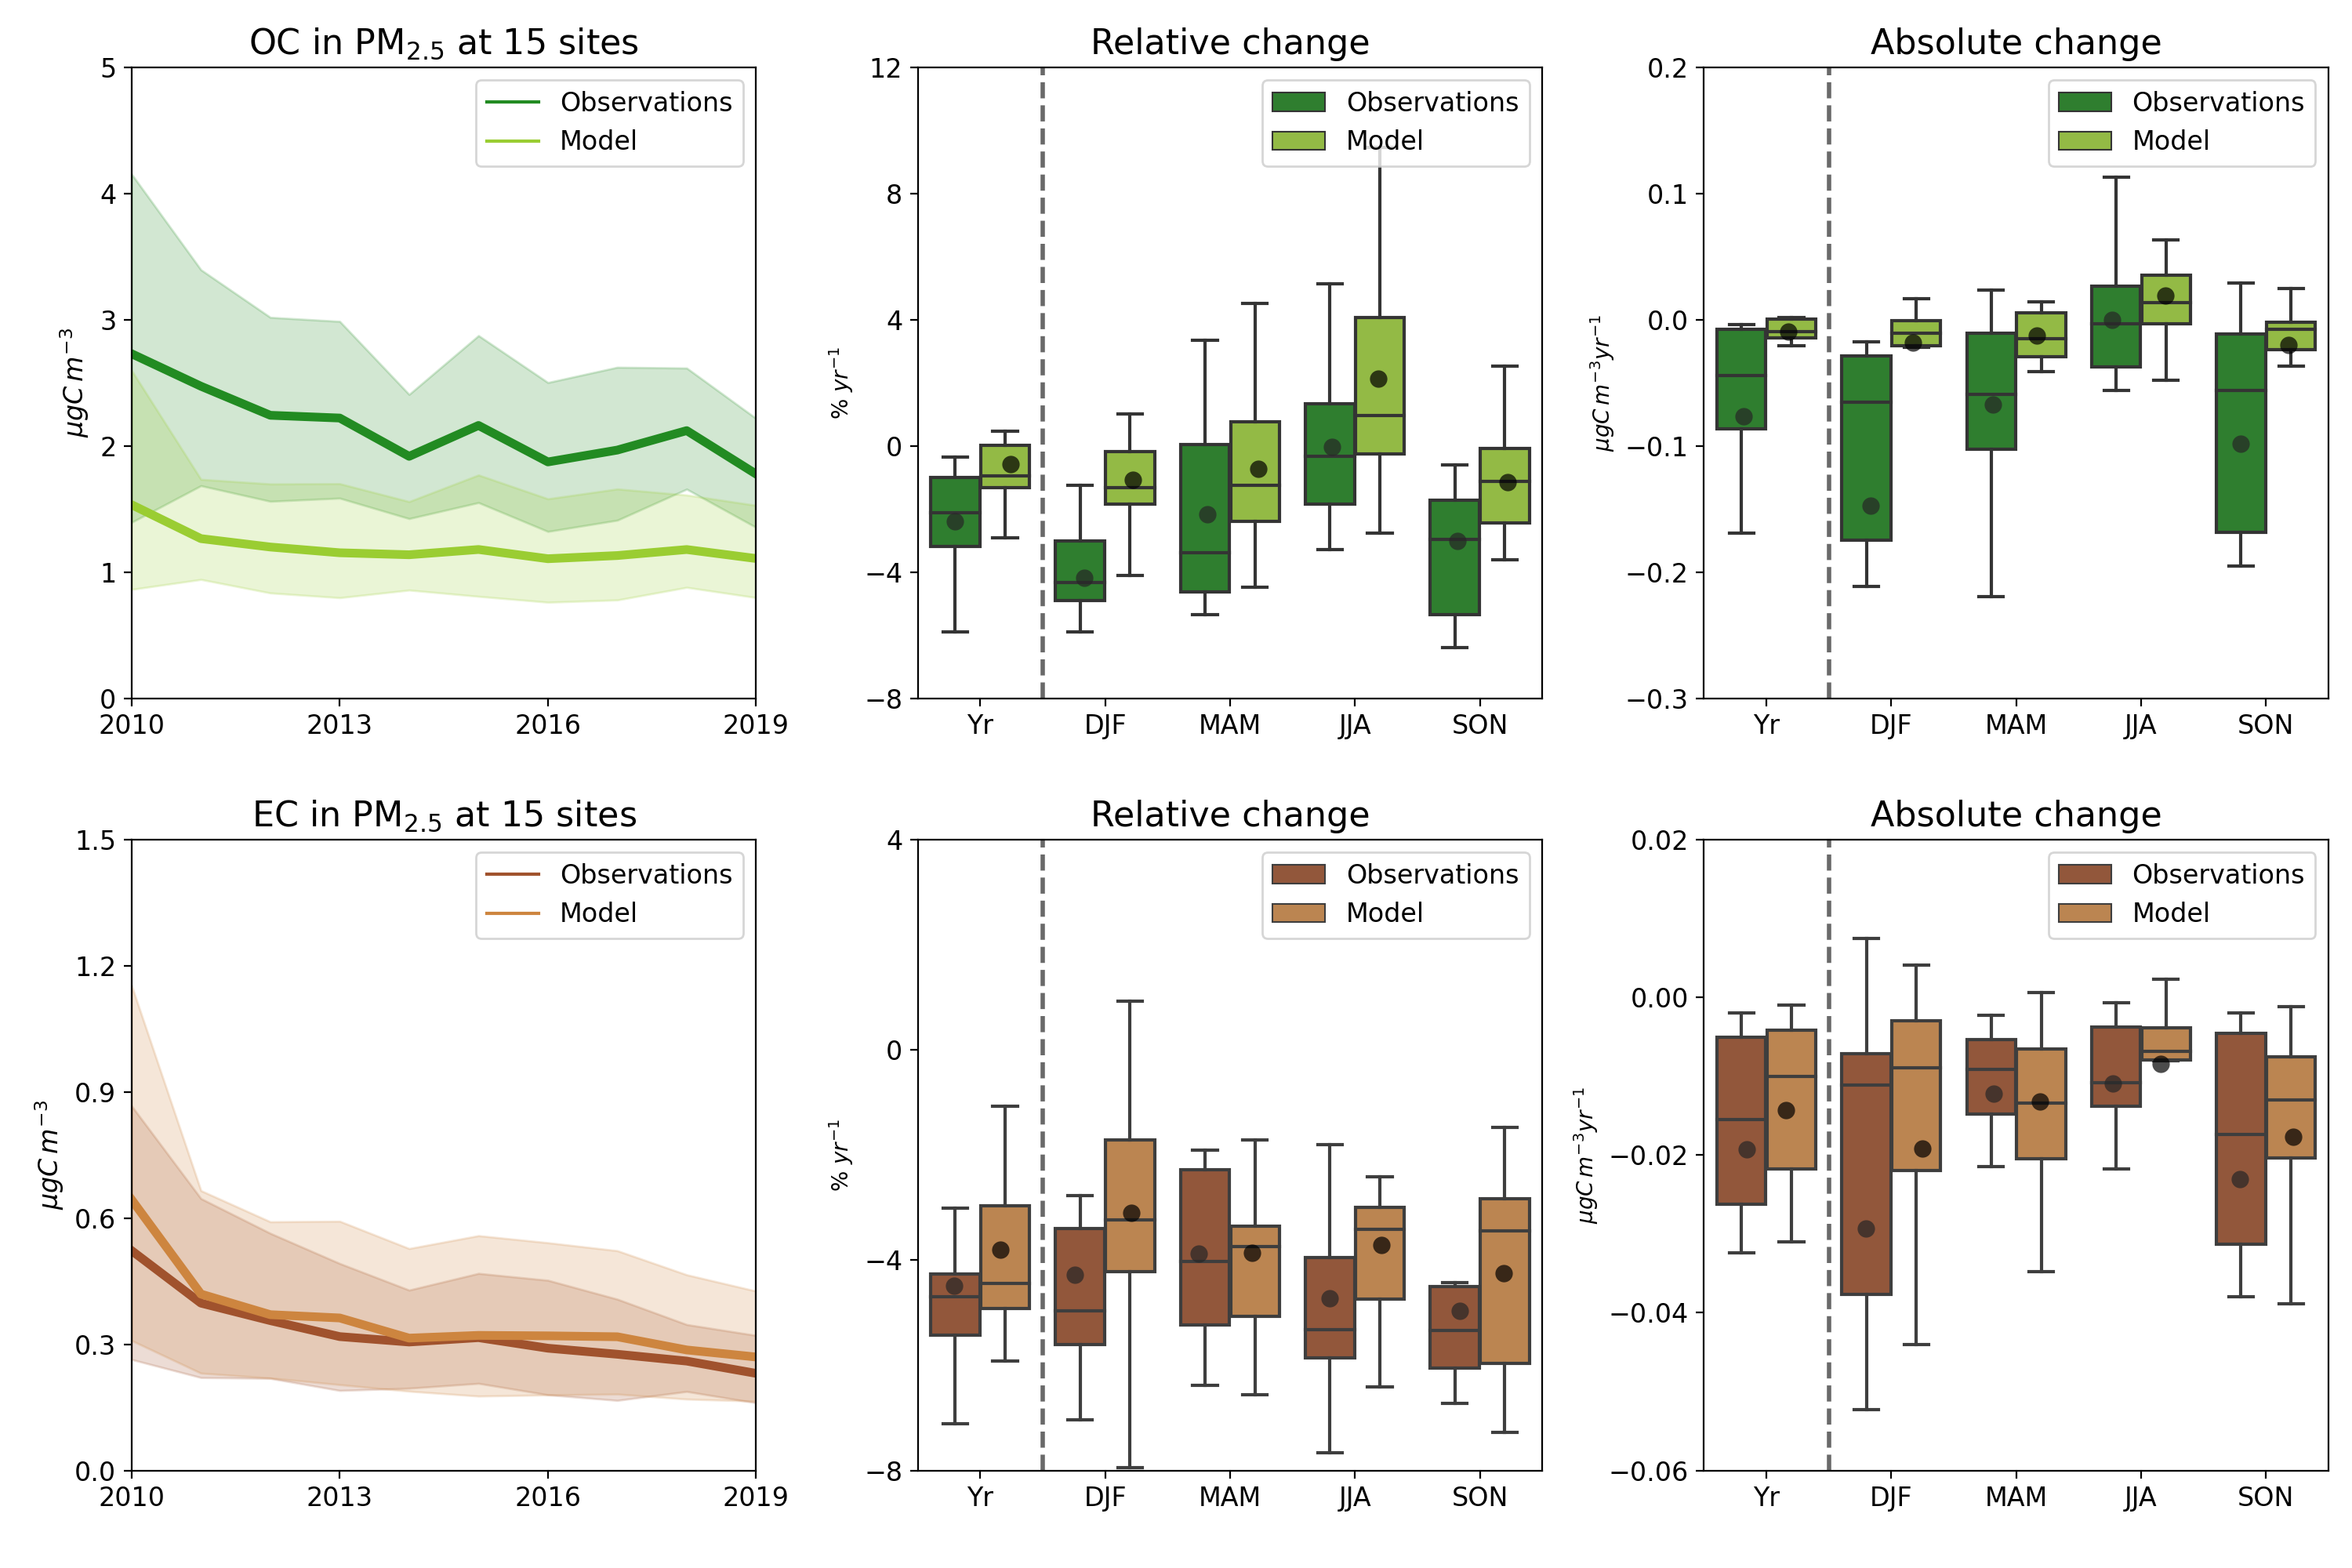
\includegraphics[width=16cm]{FIGS_TRENDS/ECOC_trends.png}
\caption{Observed and modeled concentrations and trends of EC and OC at 15 EMEP
  site across Europe for 2010--2020, showing the concentrations
  (left panels) of OC (upper) and EC (lower), aggregated annual and
  seasonal relative changes (mid panels) for OC (upper) and EC (lower),
  and aggregated annual and seasonal absolute changes (right panels)
  for OC (upper) and EC (lower). The solid line in the left panel shows
  the average annual mean for all sites and the shaded area the 95\%
  confidence interval. The box plots in the mid and right panels show
  the 25th and 75th percentiles (boxes), the median (horizontal lines),
  whereas the whiskers represent the interquartile ranges $\times$
  1.5 and the squares the outliers. Black markers within the box are
  the means.\label{fig:KEX1}
}
\end{figure}

A 4.5$\pm$1.5\%/yr reduction 
 \COMMENT{DS: changed - xx reduction to just xx reduction. Should be careful throughout...}
in elemental carbon (EC) for 2010--2020 was
calculated for the 15 sites assessed (Fig.~\ref{fig:KEX1}, Tab.~\ref{tab:KEX1}),
being quite comparable to the reduction (-5.0$\pm$0.9\%/yr)
calculated for the eleven sites where the reduction was statistically
significant. The reduction was rather similar considering these eleven
sites, ranging from -4.2\%/yr to -5.8\%/yr for ten out of eleven
sites, thus we see no apparent spatial pattern in the reductions
(Fig.~\ref{fig:KEX2}. The largest reduction was seen amongst the sites with the
highest EC levels, i.e., at Iskrba (-7\%/yr) in Slovenia and at Ispra
(-5.8\%/yr) in the Po Valley region in Northern Italy. Notably, these
were the only sites where a statistically significant reduction was
observed for all seasons, being most pronounced in summer, although
by a small margin. When considering all sites, the reduction was most
pronounced in summer and fall (Tab.~\ref{tab:KEX1}), but the general picture is
that there is a minor seasonal variability in the reduction of EC,
reflecting minor seasonal variability in most EC sources, except from
residential heating. \citet{Yttri2021} found that the reduction in EC
was most pronounced in spring and summer at the Birkenes Observatory in
southern Norway for 2001--2018, arguing that this was due to influence
from less abated sources such as domestic heating in winter and fall,
supported by a lower (-2.8\%/yr) reduction for the biomass burning
tracer levoglucosan (2008--2018) than for EC (-4.2\%/yr). Here,
we calculated a -5.2\%/yr reduction for the biomass burning tracer
levoglucosan observed at the Birkenes Observatory for 2010-2020, which is
higher than the -4.2\%/yr calculated for EC, suggesting that abatement
of carbonaceous aerosol from biomass burning has been equally successful
as that of EC from fossil fuel sources, contradicting the conclusion made
by \citet{Yttri2021} \COMMENT{DS: I would be careful with the word contradict. These time-series are not long, and as you show, one can get -2.8\% or -5.2 depending on starting year!}.   As the biomass burning emissions observed at the
Birkenes Observatory is largely long-range transported from Continental
Europe and Western Russia \citep{Yttri2021}, our finding for Birkenes
is likely to be representative for a larger part of Europe. However,
caution should be made drawing firm conclusions from such short time
series as those presented here\COMMENT{ Yes!}, illustrated by the different reductions
calculated for levoglucosan for 2008--2018 and for 2010--2020.

A statistically significant downward trend of similar magnitude
(-4.2\%/yr) was calculated for EC for 2010--2020 as for 2001--2018
for the Norwegian Birkenes Observatory \citep{Yttri2021}. Influenced by
major anthropogenic emission regions in Europe, this finding indicates a
potential for further reductions in future years not only at the Birkenes
Observatory but for Europe in general.  The model calculated a reduction
in EC of -3.9\%/yr considering all sites, which was slightly less than
for the observations (-4.5\%/yr) but highly comparable. In spring,
the model-calculated reduction equaled that based on observations,
whereas it was lower for the other seasons. As for the observations,
the model predicted a reduction in EC for all sites, but for a few sites
the model estimated a reduction that was 3--4 times larger than seen
for the observations.

\begin{table}
 \caption{Absolute change ( \ugC/yr) and relative change (\%/yr) and
  corresponding confidence intervals in observed and modelled annual
  and seasonal aggregated EC concentrations at 15 sites across Europe
  for 2010--2020. The number of sites with a significant outcome is
  provided. \label{tab:KEX1}}
% \begin{tabular}{lrrrrlrlrlrl}
%\begin{center}
\scalebox{0.70}{%
\begin{tabular}{llcc|cccc|cccc}
%\toprule
\hline
               \multicolumn{4}{c}{Number of sites} & \multicolumn{4}{c}{Average change per year (\ug $yr^{-1})$} & \multicolumn{4}{c}{Relative change per year (\% $yr^{-1}$)} \\
 Season &           total & sign.(obs.) & sign.(mod.) &                   obs. &          conf.interval &  mod. &          conf.interval &                     obs. &         conf.interval &  mod. &        conf.interval \\
%\midrule
\hline
all    &              15 &         11 &          12 &                  -0.019 &  (-0.031, -0.008) & -0.014 &  (-0.021, -0.007) &                    -4.49 &  (-5.25, -3.73) & -3.81 &  (-4.59, -3.03) \\
winter &              15 &          6 &           4 &                  -0.029 &  (-0.053, -0.006) & -0.019 &  (-0.032, -0.006) &                    -4.27 &  (-5.49, -3.06) & -3.10 &  (-4.21, -1.98) \\
spring &              15 &          5 &           8 &                  -0.012 &  (-0.018, -0.006) & -0.013 &  (-0.018, -0.009) &                    -3.88 &  (-4.67, -3.09) & -3.86 &   (-4.92, -2.8) \\
summer &              15 &          8 &          10 &                  -0.011 &  (-0.015, -0.007) & -0.008 &  (-0.013, -0.004) &                    -4.73 &  (-5.71, -3.74) & -3.71 &  (-4.59,  -2.82) \\
autumn &              15 &          8 &          11 &                  -0.023 &   (-0.036, -0.01) & -0.018 &  (-0.027, -0.009) &                    -4.96 &   (-6.03, -3.9) & -4.25 &  (-5.15,  -3.35) \\
 \hline % bottomrule
\end{tabular}
}
\end{table}



\subsection{Organic Carbon}
\label{ss:trendsOC}
 
A 2.4$\pm$1.6\%/yr reduction
 \COMMENT{DS: changed - xx reduction to just xx reduction}
 in organic carbon (OC) for 2010--2020
was calculated for the 15 sites assessed (Fig.~\ref{fig:KEX1}, Tab.~\ref{tab:KEX2}), but the
downward trend was statistically significant only for Iskrba (Slovenia)
and Ispra (Italy), which are amongst the sites with the highest OC
loading. At these two sites, the reduction was noticeably higher 
(-3.1\%/yr (Iskrba) and -5.9\%/yr (Ispra)) than for the mean of all sites. The
reduction in OC appears somewhat lower at the westernmost and northernmost
sites (Fig.\ref{fig:KEX2}). A pronounced influence of natural sources in areas
less perturbed by anthropogenic emissions, exemplified by Scandinavia,
is a possible explanation \citep{Bergstrom2012,Yttri2021}, although a
less successful abatement of anthropogenic sources cannot be excluded.

\begin{figure}

\caption{Map showing relative change (\%/yr) in observed and modeled OC (left
  panel) and EC (right panel) at 15 EMEP sites across Europe. \label{fig:KEX2}}
\end{figure}

There was a pronounced seasonal variability in the reduction observed for
OC ((Fig.~\ref{fig:KEX1}, Tab.~\ref{tab:KEX2}). In winter, the
 reduction (-4.2\%/yr) was equal to
EC (-4.3\%/yr) but only statistically significant for six of the sites,
whereas no reduction (0\%/yr) was seen in summer. Spring (-2.2\%/yr)
and fall (3.0\%/yr) are transition seasons with reductions in between
that of winter and summer and statistically significant reductions were
observed only for Ispra. Unlike EC, OC has a substantial influence from
natural sources, biogenic secondary organic aerosol (BSOA) and primary
biological aerosol particles (PBAP), which prevail in the growing season,
and which is not subject to abatement and thus is a major driver of
the seasonality seen for the trend. Thus, anthropogenic OC emissions
are likely best represented by winter-time data. Increased emissions
from domestic heating are seen all over Europe in the heating season
\citep[e.g.][]{Yttri2019} when the contribution from natural sources
is low, and is generally assumed to be poorly abated, particularly
for residential wood burning. Notably, the winter-time reduction in OC
was similar to that of EC considering all sites, and at the Birkenes
Observatory the winter-time reduction in OC (-4.1\%/yr) was only somewhat
lower than for EC (-6.4\%/yr) and levoglucosan (-4.6\%/yr), suggesting
that abatement of residential wood burning emissions has been quite
effective for Europe in general, taking into account the considerations
made about the length of the time series and the Birkenes Observatory as
an indicator of European emissions (Sect.~\ref{ss:trendsEC}).  The model calculated a
reduction in OC of -0.6\%/yr considering all sites, which was noticeably
less than for the observations (-2.4\%/yr). The model also underpredicted
the decrease calculated for the observations for each season, thereby
reproducing the seasonality in trend seen for the observations. A decrease
in observed OC was calculated for all sites, whereas the model calculated
an increase, typically <0.5\%/yr, for four of the sites.

%%%%%%%%%%%%%%%%%%%%%%%%%%%%%%%%%%%%%%%%%%%%%%%%%

\begin{table}
 \caption{Absolute change ( \ugC/yr) and relative change (\%/yr) and
   corresponding confidence intervals in observed and modeled annual
   and seasonal aggregated OC concentrations at 15 sites across Europe
   for 2010--2020. The number of sites with a significant outcome
   is provided. \label{tab:KEX2}
 }
 
%\begin{center}
\scalebox{0.70}{%
\begin{tabular}{llcc|cccc|cccc}
\hline % toprule
\multicolumn{4}{c}{Number of sites} & \multicolumn{4}{c}{Average change per year (\ug $yr^{-1})$} & \multicolumn{4}{c}{Relative change per year (\% $yr^{-1}$)} \\
Seasons &  No. & sign.(obs.) & sign.(mod.) &                    obs. &          conf.interval &  mod. &          conf.interval &                     obs. &         conf.interval &  mod. &        conf.interval \\
\hline % midrule
all    &              15 &          2 &           1 &                  -0.077 &  (-0.132, -0.022) & -0.009 &     (-0.019, 0.0) &                    -2.40 &  (-3.23, -1.57) & -0.59 &   (-1.21, 0.03) \\
winter &              15 &          6 &           1 &                  -0.148 &  (-0.249, -0.047) & -0.018 &  (-0.032, -0.004) &                    -4.19 &  (-5.16, -3.22) & -1.09 &  (-2.03, -0.15) \\
spring &              15 &          1 &           0 &                  -0.067 &   (-0.104, -0.03) & -0.013 &  (-0.023, -0.003) &                    -2.18 &  (-3.68, -0.67) & -0.74 &   (-1.94, 0.47) \\
summer &              15 &          0 &           1 &                  -0.000 &   (-0.024, 0.023) &  0.019 &   (-0.003, 0.041) &                    -0.03 &   (-1.19, 1.12) &  2.13 &    (0.44, 3.83) \\
autumn &              15 &          1 &           0 &                  -0.098 &   (-0.16, -0.037) & -0.020 &     (-0.041, 0.0) &                    -3.03 &  (-4.43, -1.62) & -1.16 &   (-2.47, 0.15) \\
\hline % bottomrule
\end{tabular}
} % end scalebox
\end{table}

%%%%%%%%%%%%%%%%%%%%%%%%%%%%%%%%%%%%%%%%%%%%%%%%%

\subsection{OC and EC fractions of PM}
\label{ss:OCECfrac}


\begin{figure}
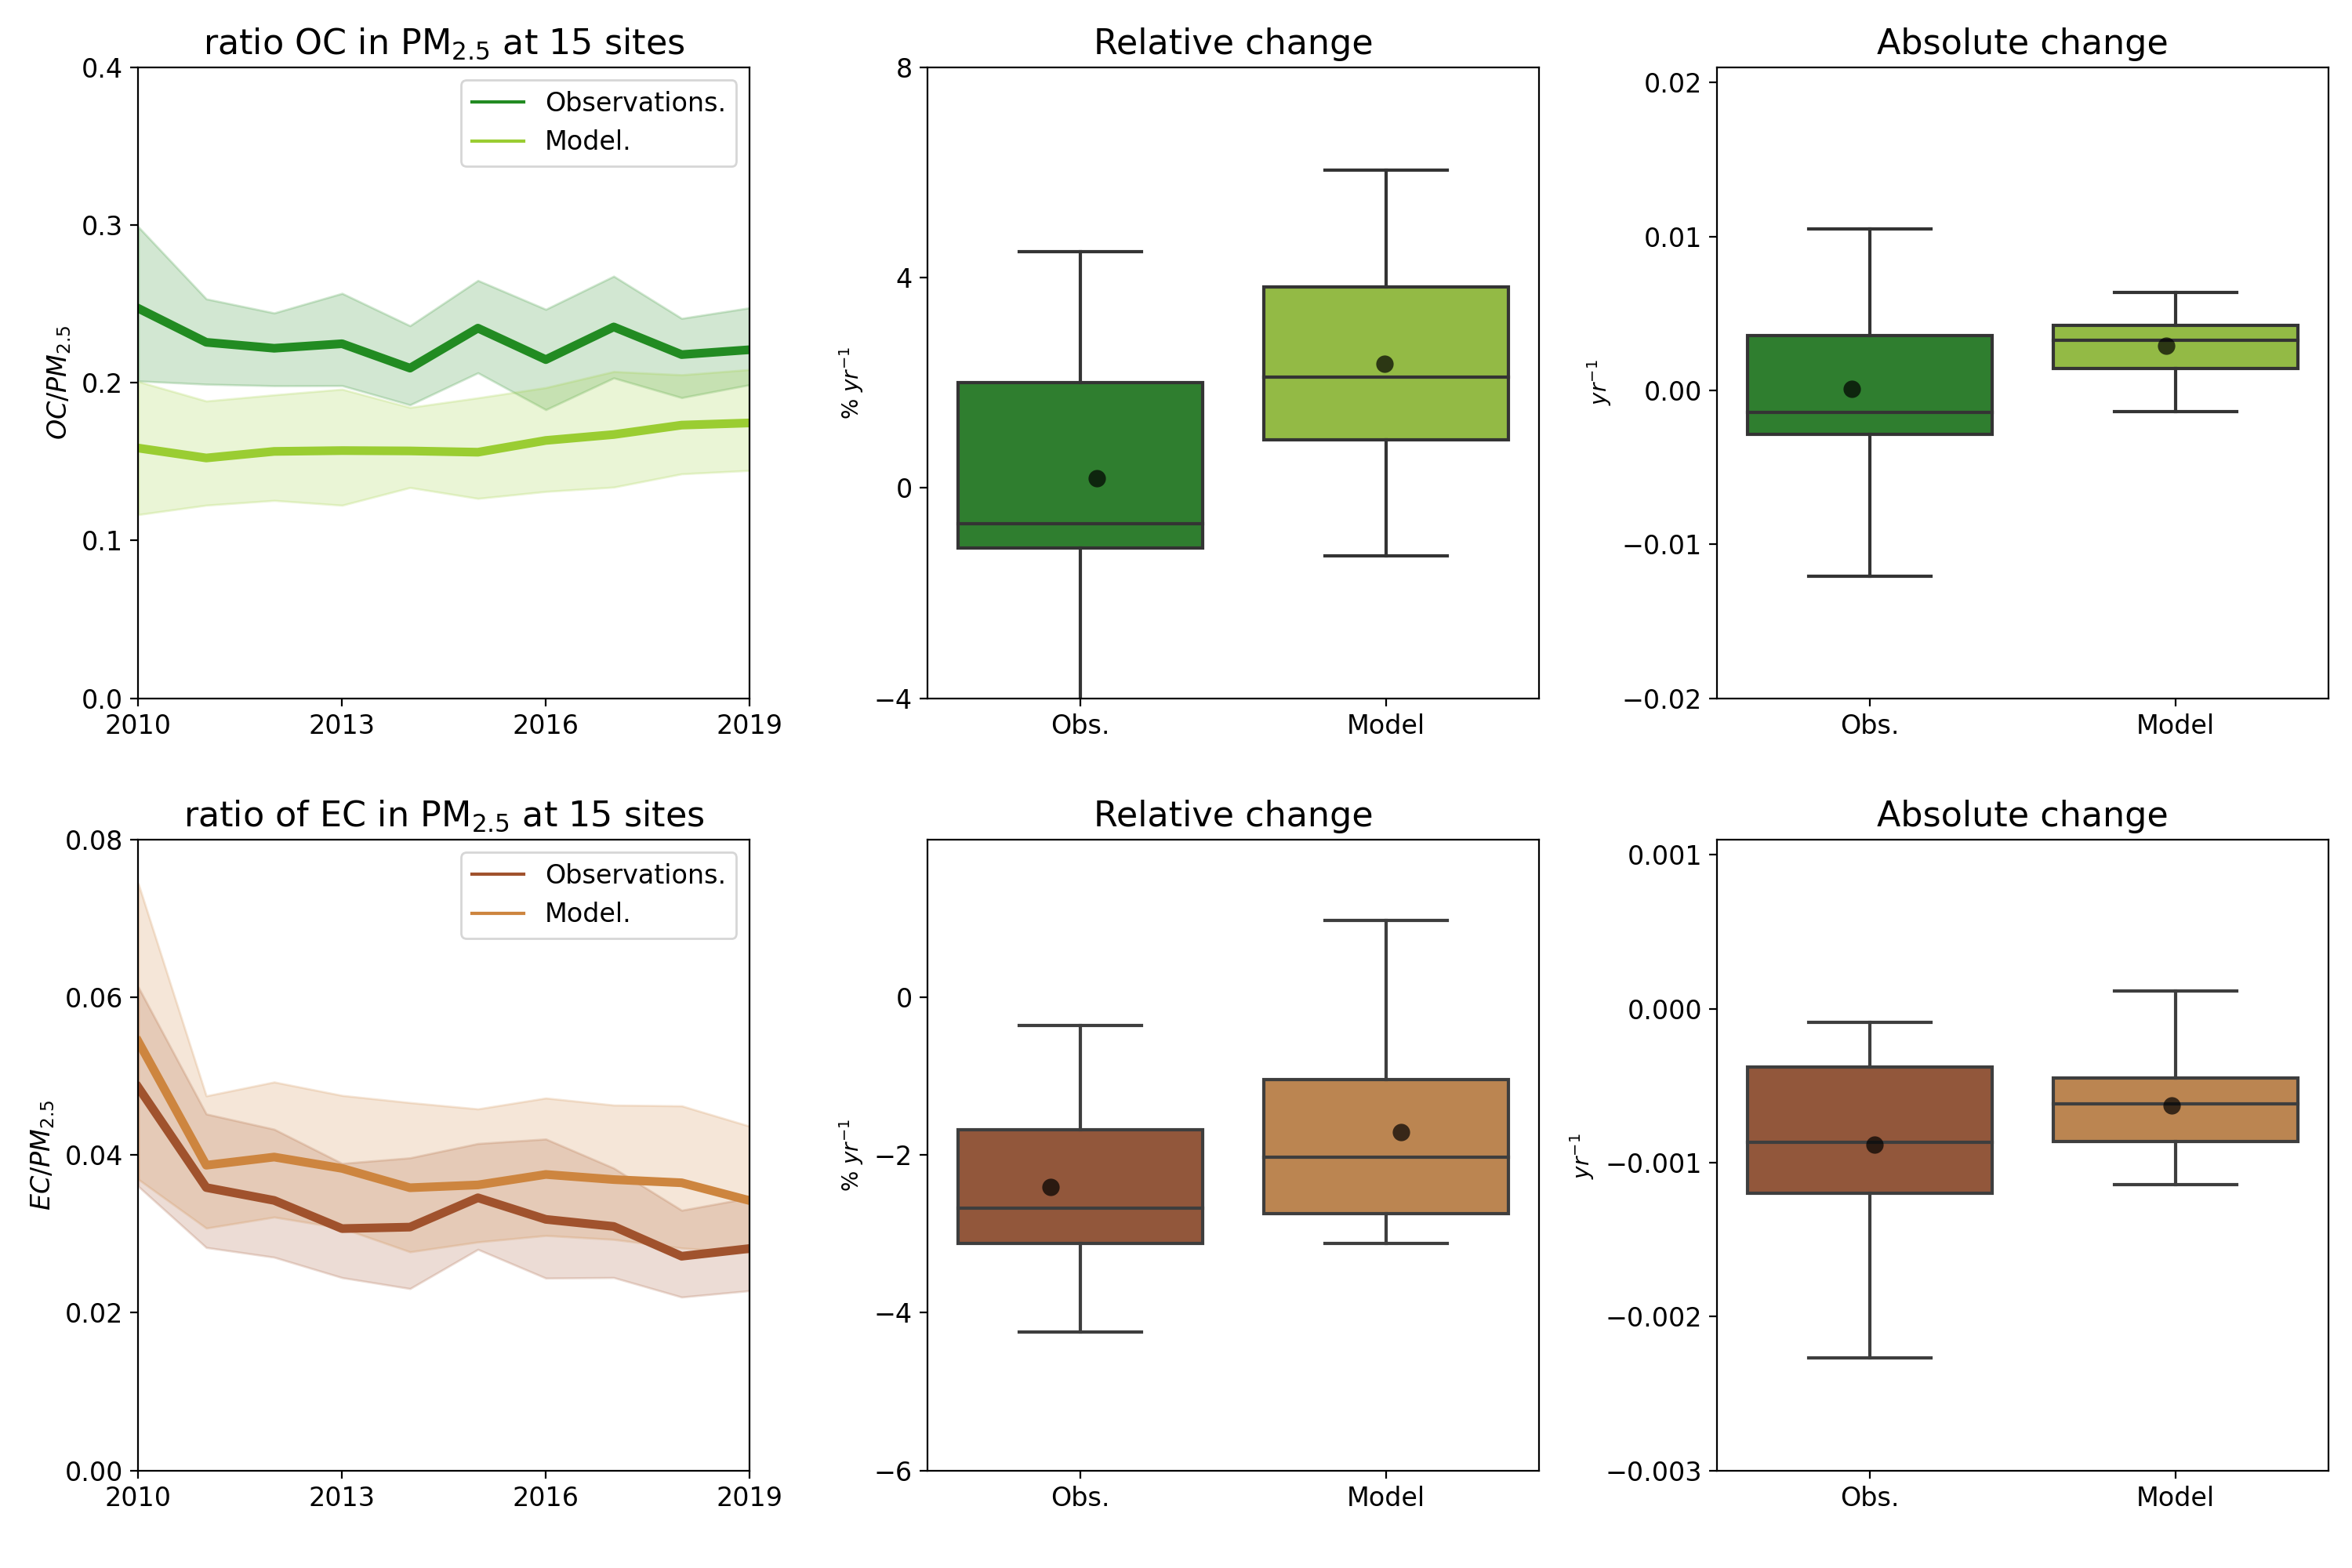
\includegraphics[width=16cm]{FIGS_TRENDS/ECOC_ratio_trends.png}
 \caption{Observed and modeled ratios and trends of OC/\pmfine and EC/\pmfine for
  15 EMEP sites across Europe for 2010--2020, showing the trends
  (left panels) of OC/\pmfine (upper) and EC (lower), aggregated annual and
  seasonal relative changes (mid panels) for OC (upper) and EC (lower),
  and aggregated annual and seasonal absolute changes (right panels)
  for OC (upper) and EC (lower). The solid line in the left panel shows
  the average annual mean for all sites and the shaded area the 95\%
  confidence interval. For explanation of the statistics in the figure,
  see Fig. X.1. \label{fig:KEX3}
 }
\end{figure}

As focused abatement of anthropogenic secondary inorganic aerosol (SIA)
precursors have reduced ambient SIA levels substantially (Sect. \QUERY{X.?}),
other, non-SIA fractions are likely to contribute an increasing fraction
of PM. For the EC fraction of \pmfine, however, there was a -2.4$\pm$1.1\%/yr
reduction for 2010--2020 (Fig.~\ref{fig:KEX3}, Tab.~\ref{tab:KEX3}), showing that EC has been
more efficiently abated than the overall PM mass concentration. The model
calculated a comparable -1.7$\pm$1.3\%/yr reduction for the EC/\pmfine ratio
but predicted a minor increase at two of the sites, which was not seen for
observed EC/\pmfine ratios. For the few sites where measurements allow for
a harmonized data set of EC, OC, \ce{SO4^2-} and \pmfine, i.e., only including
measurements on common days, the reduction in the EC fraction of \pmfine
was typically equally high or higher than for the \ce{SO4^2-} fraction. The
OC fraction of \pmfine showed no decrease or increase (0.2$\pm$2.8\%/yr)
for 2010--2020 when considering all sites, which largely is explained by
non-abatable natural sources making up a major part of OC. A substantial
4.5\%/yr increase in OC/\pmfine was calculated for the Norwegian sites,
experiencing low (anthropogenic) aerosol levels and a high OC fraction
from natural sources, thus one cannot exclude the possibility that part
of this increasing trend is due to an increase in natural sources and
not exclusively from a decrease in anthropogenic emissions. A 2.8\%/yr
increase in the OC fraction was observed for the Spanish site Montseny,
resembling the Norwegian sites with respect to a low aerosol level and
a high OC fraction from natural sources \citep{Kulmala2011}. For the
rest of continental Europe, a minor $\pm$1\%/yr increase/decrease
was seen at most sites and a $\pm$2\%/yr for a few. The Kosetice
(Czech Republic) (-5.3\%/yr) and Shauinsland (Germany) (-3.1\%/yr) sites
experienced a substantial decrease in the OC fraction, which was larger
than the corresponding decrease in the EC fraction, thus deviating from
the pattern seen at all other sites where the decrease in EC/\pmfine $>$
OC/\pmfine.

\begin{figure}
 \caption{
  Mass balance of \pmfine at Ispra (IT04), Birkenes (NO02), Diabla Gora
  (PL05) and Iskrba (SI08) including OM, EC, \ce{SO4^2-}, \ce{NO3^-}, \ce{NH4^+} and mineral
  dust (MD) (IT04 and SI08 only) (left panel) and apportionment of eBC
  into biomass burning/solid fuel (eBCbb) and fossil fuel/liquid fuel
  (eBCff) for winter 2017/2018 (right panel). \label{fig:KEX4}
 }
\end{figure}


The relative contribution of carbonaceous aerosol, OM (OM = OC $\times$
1.4--1.7)
\QUERY{DS: could be $>$2!} and EC, to the \pmfine mass concentration along with the major
SIA species illustrates the importance of the OM fraction for a further
reduction in \pmfine mass concentration (Fig.~\ref{fig:KEX4}). As a first step,
the natural and the anthropogenic fraction of the carbonaceous aerosol
must be separated, then further into abatable categories. Separation of
eBC into biomass burning/solid fuel (eBCbb) and fossil fuel/liquid fuel
(eBCff) is possible using data from the multi wavelength aethalometer,
currently available at $<$25 EMEP/ACTRIS sites across Europe \citep{Platt20XX}
\QUERY{Refs: EMEP, 2020; EMEP, 2019; EMEP, 2014}. An obvious next
step is to implement such analysis as part of regular monitoring,
making it possible to validate not only model performance, but also the
effort made in reducing carbonaceous aerosol from fossil fuel and biomass
burning sources. Although not directly comparable to the multi-year plots
presented in Fig.~\ref{fig:KEX4}, results from the EIMPs Winter 2017/2018 nicely
illustrates the split between eBCbb and eBCff for winter 2017/2018 for
the Italian site Ispra, (IT04), the Norwegian site Birkenes (NO02), the
Polish site Diabla Gora (PL05) and the Slovenian site Iskrba (SI08). The
apportionment of eBC can also be used to infer the corresponding fractions
of OM.

\begin{table}
\centering
\parbox{14cm}{
 \caption{
   Absolute change (\ugC/yr) and relative change (\%/yr) and corresponding
   confidence intervals in observed and modeled annual and seasonal
   aggregated OC/\pmfine and EC/\pmfine ratios at 15 sites across Europe
   for 2010--2020. The number of sites with a significant outcome
   is provided.\label{tab:KEX3}
 }}
 \scalebox{0.95}{%
 \begin{tabular}{lcccccc}
\hline  % toprule
 &  &  &  &  &  &  \\
\multicolumn{7}{c}{EC/\pmfine (2010--2020)} \\
  &  &  &  &  &  &  \\
  \hline
     \multicolumn{3}{c}{Number of sites} & \multicolumn{2}{l}{Average change per year} & \multicolumn{2}{l}{Relative change per year} \\
{} &           total & sign. &                     abs &       Conf. interv. &                      \%/y &   Conf. interv. \\
%How   &                 &       &                         &                     &                          &                 \\
\hline  % midrule
Model &              15 &     5 &                 -0.0006 &  (-0.0009, -0.0004) &                    -1.71 &   (-2.32, -1.1) \\
Obs.  &              15 &     4 &                 -0.0009 &  (-0.0012, -0.0006) &                    -2.41 &  (-2.96, -1.85) \\
\hline  % bottomrule
% \end{tabular}
   &  &  &  &  &  &  \\
\multicolumn{7}{c}{OC/\pmfine (2010--2020)} \\
   &  &  &  &  &  &  \\
% \begin{tabular}{lrrrlrl}
\toprule
   \multicolumn{3}{c}{Number of sites} & \multicolumn{2}{l}{Average change per year} & \multicolumn{2}{l}{Relative change per year} \\
{} &           total & sign. &                     abs &     Conf. interv. &                      \%/y &  Conf. interv. \\
%How   &                 &       &                         &                   &                          &                \\
\hline  % midrule
Model &              15 &     7 &                  0.0029 &   (0.0018, 0.004) &                     2.35 &     (1.3, 3.4) \\
Obs.  &              15 &     2 &                  0.0001 &  (-0.003, 0.0032) &                     0.19 &  (-1.24, 1.62) \\
\hline  % bottomrule
\end{tabular}
} % end scalebox
\end{table}

\subsection{Issues with inventories used in modelling}

\COMMENT{Dave will add text on condensables and EC/OC/remPPM splits - these will affect modelled trends, and add more caveats.}

\subsection{Conclusion}
\label{ss:trendsECOCconc}

A -4.5$\pm$1.6\%/yr reduction in EC was calculated across Europe for
2010--2020 and the reduction was particularly consistent amongst the
sites where the reduction was statistically significant. The model
predicted a reduction that was somewhat lower (-3.9\%/yr) than the
observations, but still comparable. A similar reduction in EC (-4.2\%/yr)
was calculated for 2010--2020 as for 2001--2018 at the Birkenes
Observatory in southern Norway. This consistent reduction indicates a
potential for further reduction in future years for Europe in general,
as LRT from continental Europe explains most EC from both fossil fuel
and biomass burning sources at the Birkenes Observatory. A  -5.2\%/yr
reduction in levoglucosan at the Birkenes Observatory (2010--2020)
 indicate that EC from wood burning in Europe is declining equally
rapid as that of EC from fossil fuel sources.

The reduction in OC (-2.4$\pm$1.6\%/yr) was less pronounced than for EC,
whereas winter-time levels (-4.2\%/yr) were comparable to EC. Non-abatable
natural sources of OC peak in the growing season diluting anthropogenic
sources, thus, anthropogenic OC emissions are likely best represented by
winter-time data. Comparable reductions in winter-time OC (-4.1\%/yr),
winter-time EC (-6.4\%/yr) and winter-time levoglucosan (-4.6\%/yr)
at the Birkenes Observatory suggest that abatement of residential
wood burning emissions has been quite effective for Europe in general,
taking into account considerations about the length of the time series
and Birkenes as an indicator of European emissions.

The model calculated a reduction in OC of -0.6\%/yr, being noticeable
less than for the observations (-2.4\%/yr). A similar underprediction
was seen for each season, thereby reproducing the seasonality in trend
seen for the observations.

The EC fraction of \pmfine (\QUERY{trend }-2.4$\pm$1.1 \%/yr) decreased at all
sites, and at a level equal as, or higher than, the \ce{SO4^2-} fraction. The
change in OC fraction was more scattered with a substantial and
consistent 4.5\%/yr increase at the northernmost sites, whereas
there was no increase or decrease (0.2$\pm$2.8\%/yr) when considering
all sites. Influence of OC from natural sources likely has a profound
impact on the general lack of decrease observed for the OC fraction of
\pmfine. These observations points to a continuous change in the aerosol
chemical composition and in the relative source composition across
Europe. The carbonaceous fraction appears particularly important for a
further reduction in the observed \pmfine mass concentration in Europe,
although effort is needed to separate its natural and anthropogenic
fraction to get a quantitative overview of the abatable fractions.


\clearpage
\bibliographystyle{copernicus}         % change bibliography-name after each
\renewcommand\bibname{References}      % bibliographystyle command!
\addcontentsline{toc}{section}{References}
\bibliography{trends,Refs,EMEP_Reports,NILU,RefsUpdates}